% Course manuscript. The editable source is deliberately independent of ReportLab.
% Compile: tectonic --keep-logs --keep-intermediates main.tex
\documentclass[conference,letterpaper]{IEEEtran}
\usepackage[T1]{fontenc}
\usepackage{amsmath,amssymb}
\usepackage{graphicx}
\usepackage{booktabs,array}
\usepackage{xcolor}
\usepackage{listings}
\usepackage[hidelinks]{hyperref}
\graphicspath{{figures/}}
% Generated by actualizar_enlaces.py from docs/enlaces_entrega.json.
\newcommand{\OverleafLink}{\textit{Pending overleaf URL}}
\newcommand{\GitHubLink}{\textit{Pending github URL}}
\newcommand{\VideoLink}{\textit{Pending video URL}}

\pagestyle{plain}
\newcommand{\NR}{\textit{not measured}}
\newcommand{\E}{\mathbb{E}}
\newcommand{\R}{\mathbb{R}}
\newcommand{\T}{^{\mathsf T}}
\lstset{basicstyle=\ttfamily\scriptsize,breaklines=true,columns=fullflexible,
 keepspaces=true,showstringspaces=false,numbers=left,numberstyle=\tiny,
 numbersep=5pt,frame=single,rulecolor=\color{black!25},xleftmargin=1.5em,
 keywordstyle=\color{blue!60!black},commentstyle=\color{black!65}}
\title{Expectation--Maximization for RSS Noise Calibration in a Synthetic Radio Tomographic Imaging Study}
\author{\IEEEauthorblockN{Camilo V\'asquez}
\IEEEauthorblockA{School of Mathematical and Computational Sciences\\
Yachay Tech University\\Urcuqu\'i, Ecuador}}
\begin{document}
\maketitle
\begin{abstract}
This course project examines Expectation--Maximization (EM) as an algorithm for estimating a two-component, zero-mean Gaussian mixture used to describe received-signal-strength (RSS) noise. A synthetic radio tomographic imaging (RTI) model provides the application context. The study separates parameter recovery from localization: EM is evaluated across five calibration sample sizes and 20 initializations, whereas classical Tikhonov RTI, a scalar Fisher-information extension, a weighted nearest-neighbor baseline, and a constant room-center control are evaluated on 500 paired generated cases. Parameter recovery generally improves with sample size under the correctly specified generating model. Mean localization errors are 3.244, 3.062, 2.618, and 2.407~m, respectively. All signal-dependent methods therefore lose to the constant control in mean error. Algebra shows that the Fisher extension merely changes the effective Tikhonov regularization from $\alpha$ to $\alpha/\gamma$; it does not provide link-specific robustness. The results support a reproducible instructional implementation of EM but do not establish useful localization, superiority over nearest neighbors, or real Wi-Fi sensing performance. The report provides the EM derivation, a numerical iteration, pseudocode, complexity analysis, traceable results, and a plan for independent development and test evaluation. The assigned EM algorithm is implemented in C++17; Python supplies data generation, RTI, validation, and plotting utilities.
\end{abstract}
\begin{IEEEkeywords}
expectation--maximization, Gaussian mixture, RSS, radio tomographic imaging, parameter estimation, synthetic evaluation
\end{IEEEkeywords}

\section{Introduction}
Radio tomographic imaging estimates changes in spatial attenuation from signal-strength changes across a network of radio links. An object may alter several links without carrying a transmitter. Wilson and Patwari formulated this setting as an ill-posed linear inverse problem and demonstrated image reconstruction using a deployed network of 28 radio nodes~\cite{wilson2010}. That application motivates this project, but its principal subject is the Expectation--Maximization algorithm, rather than the engineering of a deployable sensing system.

EM estimates parameters in models with unobserved variables by alternating a conditional-expectation calculation and a parameter update~\cite{dempster1977}. In a mixture model, the missing variable is the component that generated each observation. The observed residual is available; its component label is not. This distinction matters because estimating latent labels is different from imputing missing RSS measurements. No missing measurements are imputed in the present implementation.

The project studies a particularly small model: a mixture of two normal distributions whose means are fixed at zero. One component has a narrower spread, the other a wider spread. The parameters to estimate are one mixing probability and two standard deviations. This restricted problem is useful for an algorithms course because both steps of EM admit transparent formulas and an iteration can be checked by hand. It also illustrates initialization, convergence criteria, numerical stability, and the distinction between a fitted model and a validated application.

The application begins with a geometric matrix linking 100 image pixels to 66 radio links. Synthetic observations are generated by adding mixture noise to the attenuation predicted by that matrix. EM is fitted to a separate synthetic calibration sample. The estimated density then produces a scalar Fisher information, $\gamma$. An exploratory RTI operator inserts that scalar into regularized normal equations. This construction is explicitly distinguished from the source article's classical Tikhonov estimator and from an exact mixture-likelihood estimator.

The initial comparison contained three signal-dependent methods. Adding a constant room-center control changes the interpretation: the best signal-dependent result still has a larger mean distance error than a predictor that uses no signals. An audit must retain that result rather than selecting only the comparison in which EM appears favorable. Improving one RTI configuration is insufficient evidence that the resulting localization is useful.

This report addresses three research questions. RQ1 asks how calibration sample size affects EM recovery of known mixture parameters. RQ2 asks whether different initializations on one fixed sample give different fitted solutions. RQ3 asks what the generated localization comparison actually establishes after including a spatial control and identifying the algebraic effect of $\gamma$. These questions can be answered using the available data without claiming electromagnetic simulation, real deployment performance, or an algorithmic innovation.

The deliverable comprises a readable C++17 EM implementation, repeated calibration diagnostics, a paired synthetic localization evaluation, and editable scientific documentation. Its practical boundary is precise: no hardware, human measurements, walls, rubble, propagation solver, channel-state information (CSI), angle of arrival, or time of arrival are involved. The algorithm assigned by the course is implemented in C++; auxiliary Python utilities prepare observations and evaluate the surrounding RTI application. The student must explain that division of responsibilities together with the estimation algorithm.

\section{Background and Scope of the Evidence}
\subsection{EM and incomplete data}
Dempster, Laird, and Rubin introduced EM as a general framework for maximum-likelihood estimation from incomplete data~\cite{dempster1977}. The framework covers several forms of incompleteness. A data table may contain missing entries, but incompleteness may instead arise because the generative model includes a hidden class or state. The latter interpretation applies here. Every calibration residual is observed, and EM infers its probabilistic membership in the two noise components.

Exact EM updates do not decrease the observed-data likelihood. This useful property is weaker than a guarantee of finding the global maximum. The likelihood surface may have stationary points, flat regions, equivalent labelings, or boundary solutions. Wu's analysis distinguishes convergence of likelihood values from convergence of the parameter sequence and establishes results under explicit conditions~\cite{wu1983}. Consequently, a program must report its stopping criterion and iteration limit rather than interpreting any returned parameter vector as a certified optimum.

Fixing both means to zero removes two location parameters. It also changes the geometry of the optimization problem relative to a general Gaussian mixture. Conclusions about singularities, component collapse, or identifiability must therefore be stated for this particular model. The numerical safeguards and the ordering convention used in this project are described in Section~\ref{sec:numerical}.

\subsection{RTI and the source experiment}
Wilson and Patwari represent link-wise RSS changes by a linear model, use ellipse-based pixel weights, investigate a two-component noise mixture, derive image-error bounds, and reconstruct images with Tikhonov regularization~\cite{wilson2010}. These are separate contributions within the article. The Fisher scalar appears in the bound on estimation error. It does not appear in their later classical Tikhonov reconstruction formula.

The source experiment employed TelosB nodes using IEEE~802.15.4 in the 2.4-GHz band~\cite{wilson2010}. Sharing a frequency band does not make this network Wi-Fi: IEEE~802.11 and IEEE~802.15.4 are different radio standards. In this project, ``RSS-like'' denotes generated signal-strength residuals. It does not imply that the script simulates either standard's physical layer or acquires data from a router or a phone.

The source's noise study pools link measurements after removing each link's mean. The resulting mixture estimates were $p_1=0.548$, $\sigma_1=0.971$~dB, and $\sigma_2=3.003$~dB. The current generator adopts those published values as controlled parameters. It does not independently establish that these values describe another room, device, Wi-Fi network, or deployment. Copying parameters defines a simulation condition; it is not a new empirical measurement.

\subsection{Fingerprinting and the comparison baseline}
Fingerprint localization compares a query signal pattern with reference patterns acquired at known positions. RADAR is an early radio-frequency location system using measured signal strengths and a position database~\cite{bahl2000}. Its role here is background for fingerprinting, not evidence that the present synthetic nearest-neighbor baseline reproduces that physical system.

The implemented baseline is more precisely weighted $k$-nearest neighbors: it selects the three closest training fingerprints and forms an inverse-distance weighted average of their coordinates. Both its reference fingerprints and test observations come from the same synthetic forward model. Noise draws are independent, but the spatial grid and environment model are shared. This comparison evaluates matching under a known generated environment; it does not test generalization to an unseen building.

\subsection{What the study can establish}
The data allow direct checks of implementation arithmetic, recovery under a correctly specified generating distribution, sensitivity to sample size and initial values, and the behavior of specific reconstruction settings. They do not identify how much of the behavior would persist under channel-model mismatch. In particular, a two-variance mixture is not a complete model of multipath propagation, and generating independent wide-component samples does not demonstrate resistance to non-line-of-sight (NLoS) obstruction.

No result from recent CSI-based, multi-access-point localization work is transferred to the present experiment. Such methods can involve richer observations and different estimators. Their reported performance cannot justify a numerical accuracy claim for a fixed RSS ellipse model. The evidence chain in this report remains limited to the source RTI formulation, the standard EM framework, and the local synthetic output files.

\section{Problem Definition and Data Flow}
\subsection{Observed and unobserved quantities}
Let $r_i\in\R$ denote calibration residual $i$, for $i=1,\ldots,N$. The residual is expressed in dB and assumed to be centered at zero. Let $z_i\in\{1,2\}$ identify the latent mixture component. The unknown parameter vector is
\begin{equation}
\theta=(p,\sigma_1,\sigma_2),\quad 0<p<1,\quad 0<\sigma_1\leq\sigma_2.
\end{equation}
The ordering distinguishes the narrower component from the wider component; without it, swapping labels represents the same density.

The complete calibration data would contain both $r_i$ and $z_i$. Only $r_i$ is supplied to EM. Although the generator internally draws component labels, those labels are not used by the fitting function. The generating parameters are used later to score recovery; they are not supplied as true values to the estimator. Separating these roles prevents a trivial evaluation in which an estimator is handed the quantity it is meant to infer.

The localization experiment has a different unknown: an attenuation image $x\in\R^V$. Its observed input is a link vector $y\in\R^M$. Geometry determines a matrix $W\in\R^{M\times V}$. EM does not directly estimate the target position. Instead, its fitted noise parameters enter one exploratory reconstruction setting through $\gamma$. The classical RTI baseline and the nearest-neighbor baseline operate without fitting a latent target class by EM.

\begin{figure}[t]
\centering
\fbox{\begin{minipage}{0.92\columnwidth}\centering\small
Known mixture parameters $\theta_0$\\[2pt]
$\downarrow$ generate independent calibration residuals\\[2pt]
$r_1,\ldots,r_N\;\longrightarrow\;\text{EM}\;\longrightarrow\;\widehat\theta$\\[2pt]
$\downarrow$ evaluate fitted density and Fisher integral\\[2pt]
$\widehat\gamma$ and parameter-recovery diagnostics\\[5pt]
Known geometry $\longrightarrow W$; target pixel $\longrightarrow x$\\[2pt]
$\downarrow$ independent query noise\\[2pt]
$y=Wx+n$ to RTI, Fisher extension, and weighted K-NN\\[2pt]
$\downarrow$ same targets; independent constant-center control\\[2pt]
Distance errors, paired comparisons, and limitations
\end{minipage}}
\caption{Two connected but distinct experiments. Calibration evaluates EM parameter estimation. Localization evaluates fixed predictors on generated queries. The center control uses no query signal. All arrows denote computation, not physical radio acquisition.}
\label{fig:flow}
\end{figure}

\subsection{Independence and conditioning}
Calibration residuals, fingerprint-training noise, and query noise are separate random draws. The same query vector is passed to every signal-dependent method in a localization case. This pairing controls which noise realization each method sees. It does not make the methods identical in available information: the fingerprint method has a labeled position database, whereas RTI uses the geometric matrix and a smoothing prior.

The main localization evaluation conditions on one geometry and one fitted calibration density. Bootstrap intervals therefore describe variation across generated query cases under that fixed configuration. They do not include uncertainty from selecting another room, recollecting calibration, changing devices, or refitting the density. Keeping the conditioning explicit is essential when interpreting a narrow interval.

\subsection{Model checks before fitting real data}
Applying this pipeline to real measurements would require link-wise centering, acquisition checks, and an assessment of temporal dependence before fitting the mixture. A residual mean far from zero contradicts the fixed-mean assumption. Several links with different offset distributions may require link-specific treatment. Repeated fading intervals can make consecutive residuals dependent even when their one-dimensional histogram resembles a mixture.

The present synthetic generator deliberately avoids those complications. It supplies independent residuals from the fitting model, which is appropriate for a first implementation check. Correct performance in this setting establishes that the estimator can recover a distribution it was designed to fit. The next scientific question would be how recovery changes under departures from that model, rather than whether successful recovery already validates the sensing system.

\section{Derivation of the EM Algorithm}
\label{sec:em}
\subsection{Observed-data likelihood}
Define the zero-mean normal density by
\begin{equation}
\phi(r;0,\sigma^2)=\frac{1}{\sqrt{2\pi}\sigma}
\exp\left(-\frac{r^2}{2\sigma^2}\right).
\end{equation}
The mixture density is
\begin{equation}
f(r;\theta)=p\phi(r;0,\sigma_1^2)+(1-p)\phi(r;0,\sigma_2^2).
\label{eq:mixture}
\end{equation}
Assuming independent residuals, the observed-data log likelihood is
\begin{equation}
\ell(\theta)=\sum_{i=1}^{N}\log f(r_i;\theta).
\label{eq:ll}
\end{equation}
The difficulty is the logarithm of a sum. A component's contribution depends on all three parameters, so treating component membership as known would give incorrect parameter updates. EM resolves this by estimating probabilistic membership from the current parameters and optimizing an expected complete-data expression.

\subsection{Complete-data likelihood}
Let $s_i=1$ when $z_i=1$ and $s_i=0$ otherwise. If these indicators were observed, the log likelihood, after discarding constants independent of $\theta$, would be
\begin{align}
\ell_c(\theta)=\sum_i \bigg[&s_i\log p+(1-s_i)\log(1-p)\nonumber\\
&-s_i\log\sigma_1-(1-s_i)\log\sigma_2\nonumber\\
&-\frac{s_i r_i^2}{2\sigma_1^2}
-\frac{(1-s_i)r_i^2}{2\sigma_2^2}\bigg].
\label{eq:complete}
\end{align}
Each component now has a weighted sum of squared residuals. Because its mean is fixed at zero, the sufficient second moment is $r_i^2$, not the squared distance from a newly estimated mean. Using a general Gaussian-mixture formula that updates component means would implement a different model.

At iteration $t$, EM forms
\begin{equation}
Q(\theta\mid\theta^{(t)})=
\E_{z\mid r,\theta^{(t)}}[\ell_c(\theta)].
\end{equation}
The E-step evaluates this conditional expectation through the component responsibilities. The M-step maximizes it over the new parameters while holding the responsibilities fixed. ``Expectation'' therefore refers to the unobserved indicators conditional on data; it does not mean replacing every residual by its unconditional average.

\subsection{E-step: responsibilities}
Bayes' rule gives the probability that residual $i$ arose from the narrower component:
\begin{equation}
\tau_i^{(t)}=
\frac{p^{(t)}\phi(r_i;0,(\sigma_1^{(t)})^2)}
{p^{(t)}\phi(r_i;0,(\sigma_1^{(t)})^2)
+(1-p^{(t)})\phi(r_i;0,(\sigma_2^{(t)})^2)}.
\label{eq:responsibility}
\end{equation}
The wider component receives responsibility $1-\tau_i^{(t)}$. These numbers are soft assignments in $[0,1]$. A residual near zero is generally more compatible with the narrower density, while a sufficiently large residual tends to favor the wider one. The mixing probabilities also influence this comparison, so a responsibility cannot be inferred from residual magnitude alone.

Two residuals with the same absolute value have identical responsibilities in this model. Their signs do not distinguish components because both densities are symmetric about zero. This property offers a simple implementation check and makes the small worked example below easy to inspect.

\subsection{M-step: mixing probability}
Write $N_1=\sum_i\tau_i$ and $N_2=N-N_1$. The terms in $Q$ involving $p$ are $N_1\log p+N_2\log(1-p)$. Differentiating gives
\begin{equation}
\frac{\partial Q}{\partial p}=\frac{N_1}{p}-\frac{N_2}{1-p}=0.
\end{equation}
Solving yields
\begin{equation}
p^{(t+1)}=\frac{N_1}{N}.
\label{eq:pupdate}
\end{equation}
The new probability is the average fractional membership in component 1. It is not a count of residuals assigned by a hard threshold. This distinction avoids information loss when an observation has substantial support under both components.

\subsection{M-step: variances}
For $v_1=\sigma_1^2$, the relevant expected terms are
\begin{equation}
Q_1(v_1)=-\frac{N_1}{2}\log v_1
-\frac{1}{2v_1}\sum_i\tau_i r_i^2.
\end{equation}
Its derivative is $-N_1/(2v_1)+\sum_i\tau_i r_i^2/(2v_1^2)$. Setting it to zero, and repeating for component 2, produces
\begin{align}
(\sigma_1^{(t+1)})^2&=\frac{\sum_i\tau_i^{(t)}r_i^2}{N_1},\\
(\sigma_2^{(t+1)})^2&=\frac{\sum_i(1-\tau_i^{(t)})r_i^2}{N_2}.
\label{eq:varianceupdate}
\end{align}
The implementation stores standard deviations, so it takes square roots after updating the weighted second moments. Reporting a variance as though it were a standard deviation would change both units and the density shape. Table~\ref{tab:notation} summarizes the relevant quantities.

\begin{table}[t]
\caption{Principal quantities and their roles}
\label{tab:notation}
\centering\small
\begin{tabular}{@{}p{0.19\columnwidth}p{0.72\columnwidth}@{}}
\toprule
Symbol & Meaning and units\\\midrule
$N,I$ & Calibration sample count and iterations; dimensionless\\
$p,\tau_i$ & Mixing probability and conditional responsibility\\
$r_i,\sigma_k$ & Residual and standard deviation; dB\\
$\sigma_k^2$ & Component variance; dB$^2$\\
$M,V$ & Number of radio links and image pixels\\
$x,y,W$ & Attenuation image, RSS-change vector, geometric matrix\\
$\alpha$ & Smoothness weight in the implemented RTI operator\\
$\gamma$ & Location Fisher information of the residual density; dB$^{-2}$\\
\bottomrule
\end{tabular}
\end{table}

\subsection{Why the iteration increases likelihood}
The conditional distribution of $z$ defined by the old parameters provides a lower-bound construction for the observed log likelihood. The E-step makes that bound tight at the current parameter vector; the M-step increases its expected complete-data term. For exact maximization on a fixed admissible parameter domain, the resulting observed likelihood does not decrease~\cite{dempster1977}.

This explanation identifies what must be checked in code. The responsibilities used for every M-step update must all come from the same old parameter vector. Updating one parameter and immediately using it to recompute another responsibility inside the same iteration would no longer be the stated EM update. Likewise, comparing likelihood values from different datasets says nothing about monotonicity on a particular fit.

The implementation's probability clipping, minimum standard deviations, and finite arithmetic define a restricted numerical procedure. A likelihood trace is therefore useful for auditing the actual computation rather than relying solely on the abstract theorem. A small parameter change can occur in a flat region, and reaching the iteration limit is different from satisfying the stopping condition. Neither event alone certifies the best possible solution.

\section{Worked Iteration and Algorithm Structure}
\subsection{A numerical example}
Consider the four residuals $(-3,-1,1,3)$~dB and initial values $p=.5$, $\sigma_1=1$, $\sigma_2=3$~dB. This is a teaching example for one iteration, not one of the 500 localization cases. It can be reproduced directly with the density and update equations.

At absolute residual 1, the two unweighted densities are approximately .241971 and .125794~dB$^{-1}$. With equal mixing probabilities, their normalized ratio gives $\tau(1)=.657949$. At absolute residual 3, the densities are approximately .004432 and .080657~dB$^{-1}$, giving $\tau(3)=.052085$. Symmetry supplies the same values at negative residuals.

The effective narrow mass is $N_1=2(.657949+.052085)=1.420068$. Therefore the updated weight is .355017. The variance updates are
\begin{align}
v_1^{\rm new}&=\frac{2(.657949)(1)+2(.052085)(9)}{1.420068}
\approx1.586845,\\
v_2^{\rm new}&=\frac{2(.342051)(1)+2(.947915)(9)}{2.579932}
\approx6.878698.
\end{align}
Taking square roots yields $\sigma_1^{\rm new}=1.259700$ and $\sigma_2^{\rm new}=2.622727$~dB. The E-step favored the wide component strongly for the two large residuals, and the M-step converted those fractional memberships into a lower narrow-component probability and updated spreads.

This example also exposes a common misconception: EM does not eliminate the large residuals. They remain observed values and contribute to both parameter estimates according to their responsibilities. Nor does it relocate the target; no geometry or position variable appears in this calibration example. Explaining these two points is sufficient to distinguish the algorithmic contribution from later RTI calculations.

\subsection{Pseudocode}
Algorithm~\ref{alg:em} uses the same information flow as the implementation. The likelihood evaluation may be added to the return record, but it does not replace the documented parameter-change stopping rule.

\begin{table}[t]
\caption{Pseudocode for the restricted EM fit}
\label{alg:em}
\centering
\begin{minipage}{.97\columnwidth}\small
\textbf{Input:} finite residual vector $r$; initial $p,\sigma_1,\sigma_2$; tolerance $\eta$; floor $s_{\min}$; limit $I_{\max}$.\\
1. Validate the residual count and retain finite values.\\
2. Choose positive initial spreads and an interior weight.\\
3. For $t=1,\ldots,I_{\max}$:\\
\hspace*{.8em}a. Save the old three-parameter vector.\\
\hspace*{.8em}b. Compute both log component densities.\\
\hspace*{.8em}c. Normalize them to obtain all $\tau_i$.\\
\hspace*{.8em}d. Compute $N_1,N_2$ and update $p$.\\
\hspace*{.8em}e. Update weighted second moments and square roots.\\
\hspace*{.8em}f. Apply the spread floor; reorder labels if necessary.\\
\hspace*{.8em}g. If maximum relative parameter change $<\eta$,\\
\hspace*{1.8em}return parameters, $t$, and convergence=true.\\
4. Return final parameters, $I_{\max}$, convergence=false.\\
\textbf{Output:} fitted weight, two spreads, iteration count, flag.
\end{minipage}
\end{table}

\subsection{Time and memory complexity}
For a fixed two-component model, evaluating densities and responsibilities visits each of $N$ residuals once per iteration. Computing the two weighted sums of squared residuals has the same order. Updating the three scalars, ordering the components, and checking the stopping rule take constant work. Thus $I$ iterations require $O(IN)$ arithmetic operations. Treating the iteration count as a constant would hide a quantity that changes with tolerance, initialization, and sample configuration.

The C++ implementation stores the residual vector and a length-$N$ responsibility vector. The component densities, effective counts, and weighted squared sums can be evaluated using scalar variables during passes over those vectors. This gives $O(N)$ working memory for the implemented fit. It does not describe the memory for the RTI image operator, the fingerprint database, plots, or stored result tables. A streaming redesign could change auxiliary storage, but it is not the implementation evaluated here.

Multiple starts and repeated sample-size experiments multiply the computational work. With $S$ starts on one sample, the cost is $O(N\sum_{s=1}^S I_s)$; for a rough common iteration count it is $O(SIN)$. With several sample sizes and repeated draws, the workload adds over those fits. These distinctions explain why a short core function can still be called many times by a longer experiment driver.

The derivation does not assume that every EM iteration is equally fast on every machine. Compiler settings, memory allocation, loop implementation, and memory traffic affect measured time. Calling the C++ process through a Python adapter also adds interface overhead that is distinct from the E-step and M-step. Complexity describes scaling of the algorithmic work. A reproducible timing study would need a separate protocol, whereas the current report avoids claiming a speed advantage from one local measurement.

\section{Numerical Implementation}
\label{sec:numerical}
\subsection{Stable normalization}
Directly evaluating exponentials can underflow for a residual that is large relative to a component spread. The implementation first computes
\begin{equation}
a_{ik}=\log p_k-\tfrac12\log(2\pi\sigma_k^2)
-\frac{r_i^2}{2\sigma_k^2}.
\end{equation}
With $m_i=\max(a_{i1},a_{i2})$, the responsibility is evaluated as
\begin{equation}
\tau_i=\frac{\exp(a_{i1}-m_i)}
{\exp(a_{i1}-m_i)+\exp(a_{i2}-m_i)}.
\end{equation}
Subtracting the same maximum cancels algebraically in the ratio while keeping the largest exponent at zero. The observed log density can similarly be computed as $m_i+\log\{\exp(a_{i1}-m_i)+\exp(a_{i2}-m_i)\}$. This implements the same statistical model with more stable arithmetic.

\subsection{Initialization, labels, and stopping}
The default mixing weight begins at .7. The initial narrow spread is .55 times the empirical sample spread, bounded below by .15~dB. The wider spread begins at 1.8 times that spread estimate and is kept larger than the narrow initial value. The diagnostic additionally supplies randomized initial values to the same fitting routine. These are initialization rules, not estimated physical constants.

At each iteration the code computes the maximum relative parameter change, using a small denominator safeguard when an old value is near zero. The fit is declared converged when this value is below $10^{-7}$; otherwise it stops at the configured iteration limit. The report distinguishes a returned estimate from the convergence flag. A nonconverged fit may still have reasonable parameters, but it should not be silently counted as a successful stopping event.

After an M-step the components are ordered by spread. If the labels swap, the mixing weight is replaced by $1-p$ to preserve the represented density. This avoids treating the same solution under opposite labels as two different recovered parameter vectors. The ordering does not force well-separated components: two estimated spreads can still become close, in which case the mixture has little practical distinction between its components.

\subsection{Floors and the zero-mean restriction}
The program restricts standard deviations to at least .15~dB and keeps mixing probabilities away from exact zero and one. These choices protect divisions and define an admissible numerical domain. They can affect a fit near the boundary, so their values should be recorded rather than treated as an invisible implementation detail.

In a Gaussian mixture with freely estimated means, the likelihood can become unbounded when one component collapses onto an observation. That generic explanation must be qualified for the model used here: both means are fixed at zero. For a fixed nonzero residual $r$, maximizing $\phi(r;0,\sigma^2)$ over $\sigma>0$ gives
\begin{equation}
\sup_{\sigma>0}\phi(r;0,\sigma^2)
=\frac{\exp(-1/2)}{\sqrt{2\pi}|r|}<\infty.
\end{equation}
Every mixture density at that nonzero residual is bounded by the same maximum. If all sample values are nonzero, their likelihood is therefore bounded, even without movable means. An exact zero changes the situation: a positive-weight component centered at zero can have density diverging as its spread approaches zero while the other component explains the remaining observations.

Thus the floor is retained as a numerical and modeling restriction, including protection for exact zeros that may occur after RSS quantization or centering. The project does not claim that a free-mean singularity occurs at an arbitrary nonzero observation in its own fixed-mean model. Sensitivity to the floor remains a future experiment; it is not measured by the current sample-size comparison.

\subsection{Separation between core and experiment driver}
The standalone \texttt{em.cpp} source contains the assigned E-step and M-step using explicit loops and standard C++17 facilities. It is compiled with \texttt{g++}; an auxiliary \texttt{em\_cpp.py} adapter supplies residuals and reads the returned parameters. The main calibration fit, sample-size diagnostics, and initialization diagnostics use that compiled backend. Geometry, random-data generation, RTI reconstruction, bootstrap summaries, and plotting remain Python utilities outside the assigned EM core.

The C++ core in Appendix~\ref{app:code} is taken from the editable source packaged with this report. Command-line parsing and the presentation demo surround that function in the full source; they are not additional EM steps. The Python implementation is retained as a reference for numerical cross-checks, rather than silently substituted for the selected C++ backend. This boundary lets the student defend the estimation loop independently of the longer experimental driver.

\section{Synthetic RTI and Comparison Methods}
\subsection{Geometry and forward model}
The room is a 6.4-m square with 12 evenly spaced perimeter nodes. Every node pair supplies an available undirected link, giving $M=12(11)/2=66$. The area is divided into a $10\times10$ grid, so $V=100$ and each pixel is .64~m wide. The count of links is smaller than the count of unknown pixels; the inverse problem therefore requires additional structure.

Let $d_l$ be the distance between a link's nodes, and $d_{lj}^{(1)}$, $d_{lj}^{(2)}$ the distances from pixel center $j$ to the two endpoints. The implemented ellipse weights follow the source-style rule
\begin{equation}
W_{lj}=\begin{cases}d_l^{-1/2},&d_{lj}^{(1)}+d_{lj}^{(2)}<d_l+\lambda,\\0,&\text{otherwise},\end{cases}
\end{equation}
with $\lambda=.10$~m. This matrix is a statistical sensitivity model. It is not a numerical solution to Maxwell's equations and does not compute reflection, material penetration, diffraction, or packet decoding.

The true image has one nonzero pixel with attenuation 4~dB. A query is generated by
\begin{equation}
y=Wx+n,
\label{eq:forward}
\end{equation}
where each element of $n$ is an independent mixture draw. This single-pixel target simplifies attribution of localization error but does not represent a complete human attenuation pattern. The source article's physical image experiment and evaluation used a different target representation and acquisition process~\cite{wilson2010}.

\subsection{Classical Tikhonov baseline}
Let $D_x$ and $D_y$ denote adjacent-grid difference operators and define $L=D_x\T D_x+D_y\T D_y$. The baseline reconstructs
\begin{equation}
\widehat x_T=(W\T W+\alpha L+\epsilon I)^{-1}W\T y,
\label{eq:tikhonov}
\end{equation}
with $\alpha=.10$ and a small numerical stabilizer $\epsilon=10^{-8}$. The image is clipped below zero, and the coordinate of its maximum is the predicted target location. Clipping is an explicit postprocessing choice; it is not the exact solution of a separately optimized nonnegative constrained problem.

For the default grid the script precomputes the dense linear operator. Inference then multiplies that operator by each query vector. The setup includes matrix construction and factorization or inversion, whereas inference applies an already prepared operator. These phases must not be mixed when discussing computational cost. At larger grids, the driver can use an iterative solver, which has a different setup and per-query profile.

\subsection{Fisher scalar and exploratory extension}
For a location-noise density $f$, the scalar Fisher information is
\begin{equation}
\gamma=\int_{-\infty}^{\infty}\frac{[f'(u)]^2}{f(u)}\,du.
\label{eq:gamma}
\end{equation}
Under the noise assumptions in the source, the data-information matrix is $J_D=\gamma W\T W$. The article combines this term with prior information to form an image-error bound~\cite{wilson2010}. A bound on possible estimation error is not itself an image estimator.

The project's exploratory operator is
\begin{equation}
\widehat x_F=(\gamma W\T W+\alpha L+\epsilon I)^{-1}\gamma W\T y.
\label{eq:fisheroperator}
\end{equation}
For positive $\gamma$, dividing the normal equations by it gives the exact identity
\begin{equation}
\widehat x_F=\left(W\T W+\frac{\alpha}{\gamma}L+
\frac{\epsilon}{\gamma}I\right)^{-1}W\T y.
\label{eq:equivalence}
\end{equation}
Consequently, this operator belongs to the same scalar Tikhonov family. Its main calibration produces $\gamma=.4182318686$, giving $\alpha/\gamma=.2391018$ rather than .10. The comparison changes the amount of smoothing. All links share the same scalar multiplier, so this construction does not identify or downweight a particular contaminated link.

The equivalence survives the subsequent common clipping and argmax operations because the reconstructed vectors are equal under the corresponding parameters. A future tuned comparison must include the baseline at $\alpha=.2391018$, with the corresponding stabilizer, as an algebraic control. Calling the present operator an exact mixture maximum-likelihood or robust NLoS estimator would misdescribe what the code computes.

\subsection{Weighted nearest neighbors and center control}
For each grid cell the driver creates three noisy reference fingerprints using the same $W$ and attenuation model. The query's nearest three vectors are selected by Euclidean signal distance. Their coordinates are averaged with inverse-distance weights, using a small distance safeguard. The label KNN in result files is retained for consistency; the report identifies its weighted prediction rule explicitly.

The constant control always returns the geometric room center $(3.2,3.2)$~m. It has no training data, no radio observations, and no calibration parameters. For uniformly sampled positions in a bounded square, it provides a meaningful check against location predictions that are effectively dispersed or uninformative. It is evaluated on exactly the same target cases as the signal-dependent methods.

Using this control does not imply that a fixed center is a usable tracking system. It instead establishes a minimum diagnostic standard for the mean-distance metric: a complex method should demonstrate value beyond the bounded geometry alone before an application claim is made. Other downstream objectives, such as multiple-person detection, remain outside this experiment.

\section{Experimental Design and Metrics}
\subsection{Calibration recovery experiment}
The generating distribution uses $p=.548$, $\sigma_1=.971$, and $\sigma_2=3.003$~dB. Five calibration sizes are evaluated: 100, 500, 1,000, 5,000, and 10,000. Each size has 20 independent replicates. For each parameter $\theta_k$, recovery is summarized by
\begin{equation}
\operatorname{MAE}(\widehat\theta_k)=\frac{1}{20}\sum_{b=1}^{20}
|\widehat\theta_{k,b}-\theta_{k,0}|.
\end{equation}
The convergence rate is the fraction meeting the parameter-change stopping rule before the limit. A larger sample can reduce estimation error without uniformly reducing the number of EM iterations. These are different outcomes and are reported separately.

This experiment evaluates recovery of a known, correctly specified density. It does not compare EM with another parameter optimizer, estimate the model's real-data goodness of fit, or demonstrate that a two-component model is preferable to a one-component model in a new environment. Such claims would require their own objective, competing fits, and held-out measurements.

\subsection{Initialization experiment}
A separate fixed calibration sample is fitted from 20 random starts. For each start, the stored diagnostics contain initial values, final estimates, iterations, convergence flag, likelihood per sample, and floor hits. Since the dataset stays fixed, variation in these fits concerns initialization rather than variation from collecting another dataset.

Ordering the components before comparing final values avoids an artificial label-switching difference. Agreement of final values and likelihoods is evidence that the chosen starts reach nearly the same solution for this sample. It is not a proof that all initializations or all possible datasets have the same behavior. Boundary starts, nearly identical component spreads, and very short calibration sequences are not exhaustively explored.

\subsection{Localization experiment}
The main run uses seed 7, 5,000 calibration residuals, and 500 target pixels sampled uniformly with replacement. Every target has an independent noisy query. All signal-dependent methods receive the same query in a case, and the center control is scored against the same target. Sampling with replacement allows repeated pixels; the 500 cases are not 500 distinct locations or physical acquisition sessions.

For case $j$ with true coordinate $q_j$ and predicted coordinate $\widehat q_j$, the error is $e_j=\|\widehat q_j-q_j\|_2$. The reported metrics are
\begin{align}
\overline e&=\frac{1}{T}\sum_{j=1}^{T} e_j,\\
\operatorname{RMSE}_{\rm position}&=\sqrt{\frac{1}{T}\sum_{j=1}^{T}e_j^2}.
\end{align}
Both are measured in meters. RMSE emphasizes larger errors more strongly. For the two image reconstructors the output also records mean pixel-wise squared image error in dB$^2$. A coordinate-only predictor has no corresponding reconstructed image, so its map error is left undefined rather than set to zero.

\subsection{Bootstrap uncertainty and paired differences}
Mean-error intervals are calculated by resampling case indices with replacement and taking percentile bounds from bootstrap means. For a comparison of methods A and B, each bootstrap sample reuses the same indices for both methods. The case difference is $d_j=e_{A,j}-e_{B,j}$, so a positive mean difference favors B.

Resampling methods independently would discard their pairing and answer a less precise question about the same generated cases. However, pairing does not remove model bias. The resulting intervals remain conditional on the fixed geometry, calibration fit, generating model, and reference database. A claim about future buildings would require replication across buildings or a defensible hierarchical sampling model.

The center control was added during audit because it materially changes interpretation. This is transparent retrospective analysis, not a prospectively registered success test. The same cases and earlier metric values are preserved. Before a confirmatory follow-up, the outcomes, development/test split, comparison methods, and decision criteria should be fixed in advance.

\subsection{Provenance of the local run}
All numerical values in the Results derive from the current \texttt{results/python\_preliminary} directory: \texttt{parametros.json}, \texttt{metricas.csv}, \texttt{em\_sample\_size.csv}, \texttt{em\_initialization.csv}, \texttt{predicciones.csv}, and \texttt{comparaciones\_pareadas.csv}. The report does not merge separate multipath pilots or historical output folders with this evaluation.

The main parameter file records the selected C++ EM backend and its compiler/source information alongside Python, NumPy, Matplotlib, and the Windows execution environment used by the auxiliary driver. The recorded compiler is \texttt{g++} 16.1.0, with C++17, optimization, warning, and static-linking flags retained in the backend manifest. These records describe the executed pipeline, not a claim that the whole RTI application has been ported to C++. The seed and configuration support rerunning the synthetic computation, while saved case-level predictions allow the metrics to be checked without regenerating the random stream. Software versions do not imply identical wall-clock measurements elsewhere.

\section{Results}
\subsection{Parameter recovery as sample size increases}
Table~\ref{tab:sample} and Fig.~\ref{fig:recovery} summarize the 20 replicates at each size. The MAE of $p$ decreases from .1048 at $N=100$ to .01095 at $N=10{,}000$. The corresponding standard-deviation MAEs decrease from .1671 to .01489~dB for the narrower component and from .4036 to .03252~dB for the wider component. This is the strongest direct result about EM in the current study: under the generating model, larger calibration samples generally recover its parameters more accurately.

The sequence is not strictly monotonic for every parameter. For example, the $p$ MAE at $N=1{,}000$ is slightly larger than at $N=500$. With only 20 repetitions per size, such fluctuation should not be described as an algorithmic reversal. A smooth trend through the five points is a visual summary, not a measured convergence-rate law in $N$.

At $N=100$, 19 of 20 fits meet the stopping rule. All fits do so at the four larger sizes. This convergence flag concerns parameter stability, not exact agreement with the generating parameters. The average iteration counts are 182.25, 147.6, 159.5, 144.6, and 141.9, respectively. Increasing sample size therefore reduces recovery error much more clearly than it orders computational iteration counts.

\begin{table}[t]
\caption{EM recovery over 20 independent replicates per size}
\label{tab:sample}
\centering\small
\begin{tabular}{@{}rrrrr@{}}
\toprule
$N$ & Conv. & MAE $p$ & MAE $\sigma_1$ & MAE $\sigma_2$\\
& rate & & (dB) & (dB)\\\midrule
100 & .95 & .10478 & .16715 & .40361\\
500 & 1.00 & .03751 & .05091 & .12299\\
1,000 & 1.00 & .03811 & .05010 & .11400\\
5,000 & 1.00 & .01575 & .01944 & .04785\\
10,000 & 1.00 & .01095 & .01489 & .03252\\
\bottomrule
\end{tabular}
\end{table}

\begin{figure*}[t]
\centering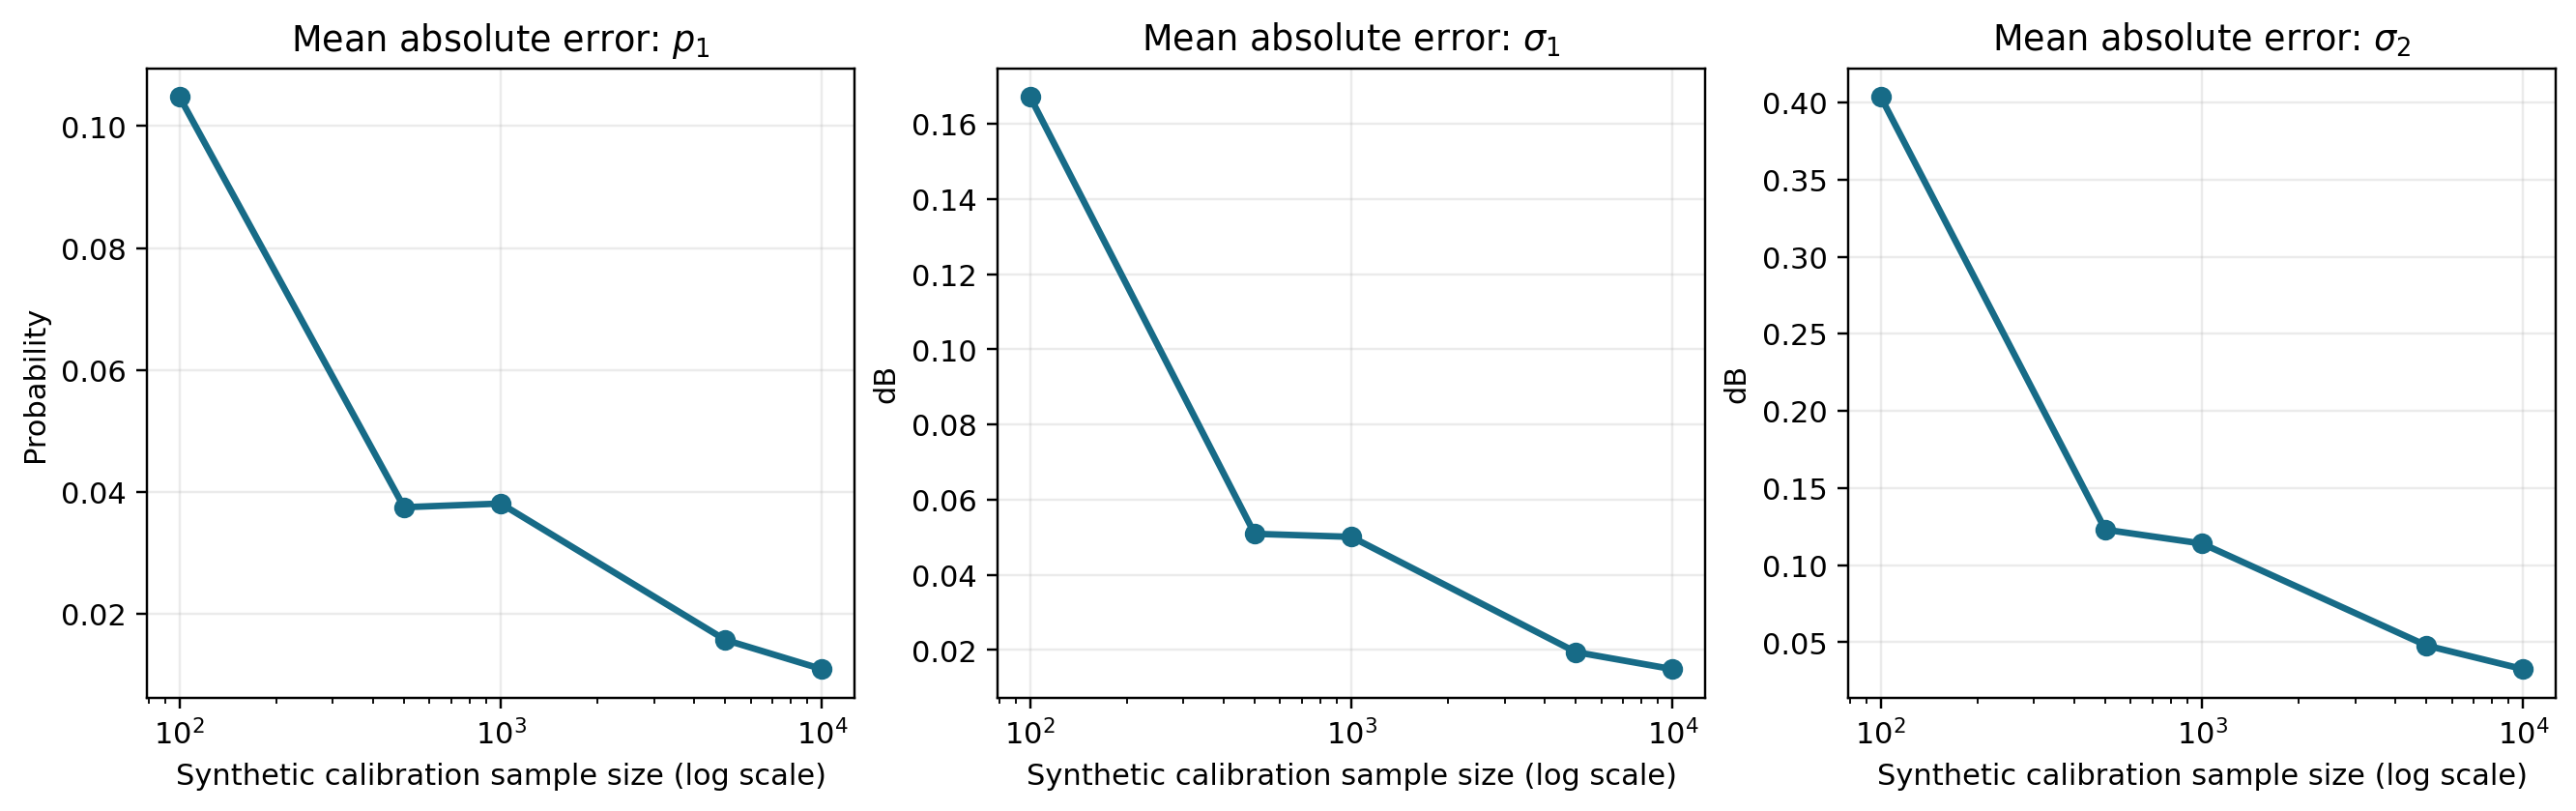
\includegraphics[width=.94\textwidth]{em_parameter_recovery.png}
\caption{Parameter-recovery MAE from 20 synthetic fits at each calibration size. Each parameter is scored against its generating value. Curves summarize a finite experiment; they do not establish a universal sample-complexity bound or performance on measured RSS. Source: \texttt{em\_sample\_size.csv}.}
\label{fig:recovery}
\end{figure*}

\subsection{Main fit and initialization sensitivity}
The 5,000-residual main fit gives $\widehat p=.5618915$, $\widehat\sigma_1=.9704574$, and $\widehat\sigma_2=2.9933068$~dB. It satisfies the stopping rule after 145 iterations. Its numerical Fisher information is .4182318686~dB$^{-2}$. These values are estimates for one generated calibration sample and need not equal the parameters used to generate the sample exactly.

The initialization diagnostic uses another fixed sample. Across 20 starts, the fitted values are nearly identical: approximately $p=.5347$, $\sigma_1=.9163$, and $\sigma_2=2.8911$~dB, as shown in Fig.~\ref{fig:starts}. Likelihoods per sample also agree within numerical rounding. The difference from the main fit follows from using a different calibration sample; it is not a contradiction or a repeated fit of the same residuals.

Agreement across these starts supports reproducibility with respect to the tested initializations. It does not justify calling the estimate globally optimal. The source convergence theory requires conditions on the objective and parameter sequence; trying 20 points cannot establish those conditions for every possible sample~\cite{wu1983}. The diagnostic is evidence of practical behavior within its stated range.

\begin{figure*}[t]
\centering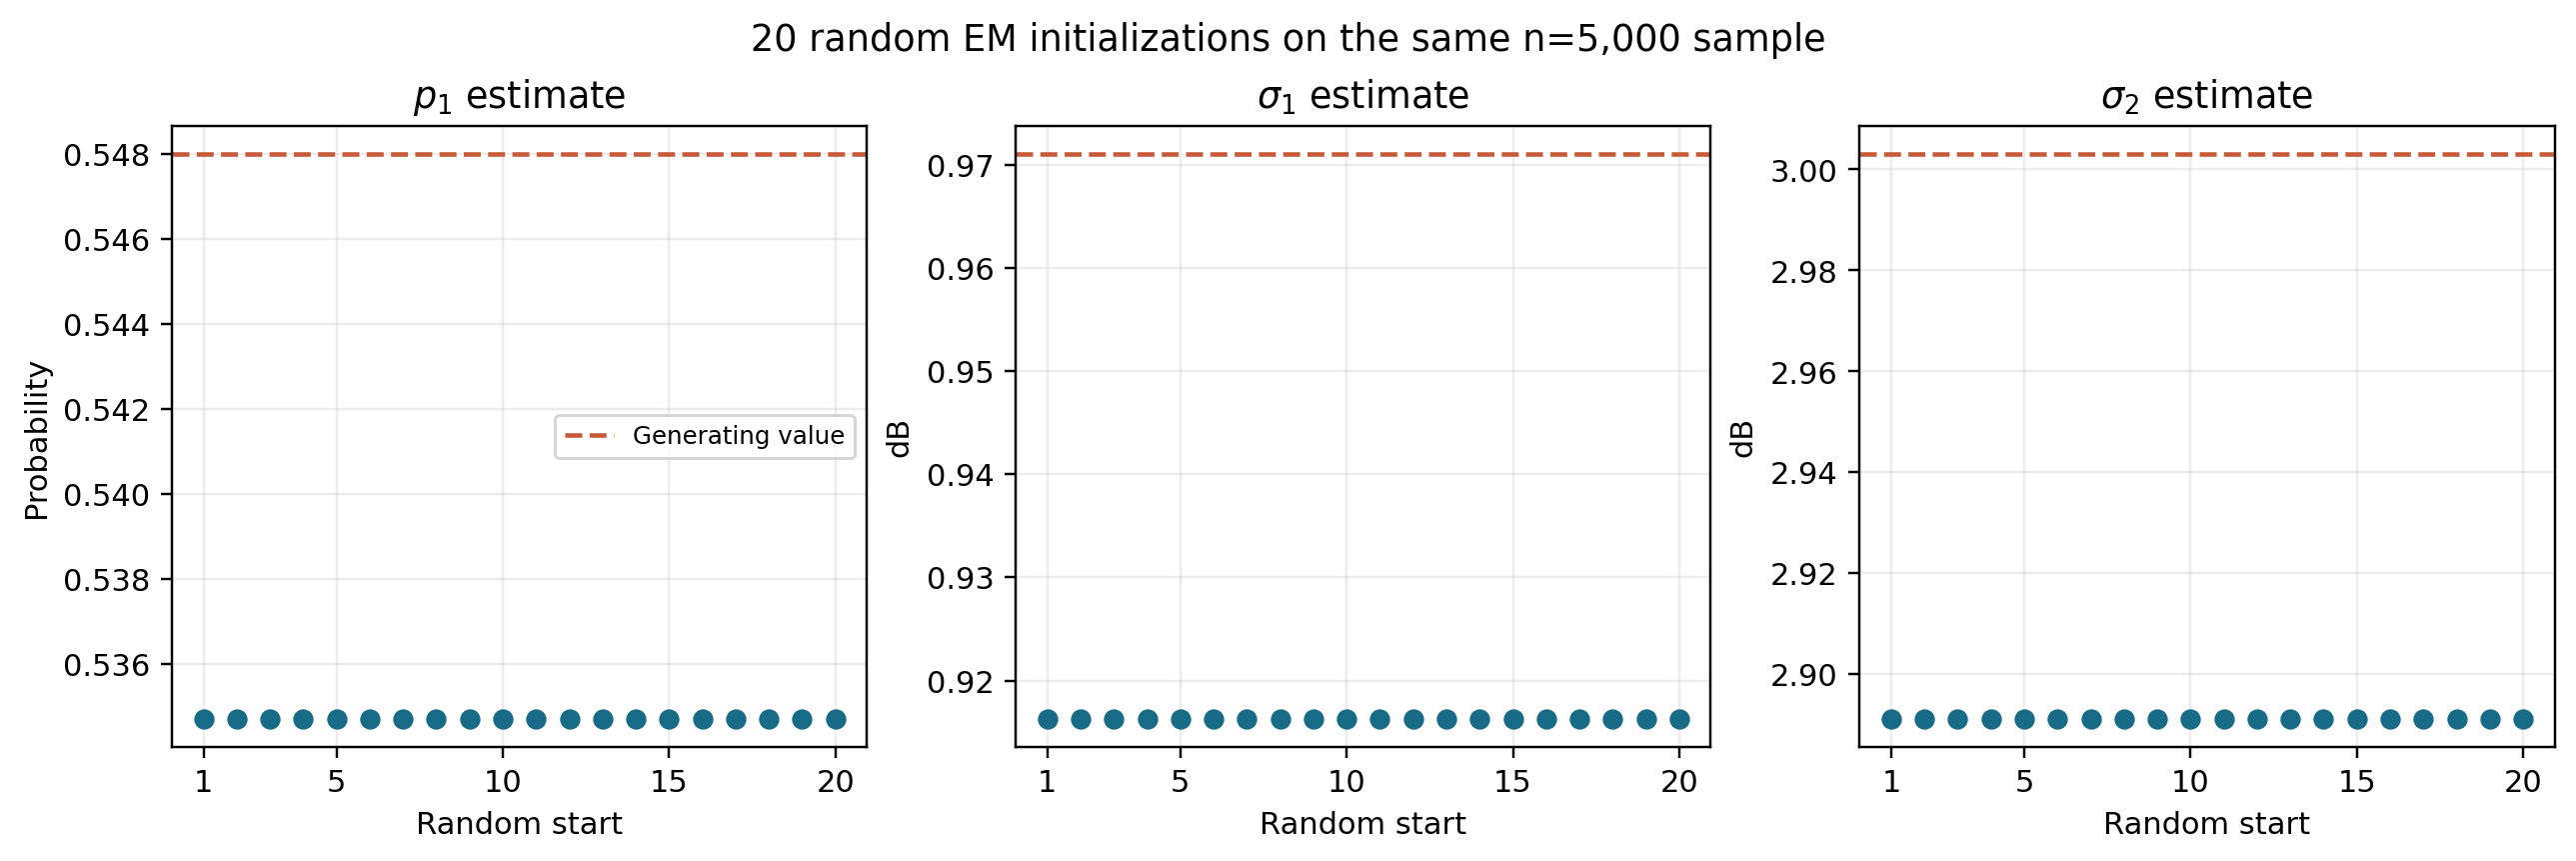
\includegraphics[width=.94\textwidth]{em_initialization_sensitivity.png}
\caption{Final estimates from 20 starts on one fixed synthetic calibration sample. Dashed lines denote generating parameters. Their difference from the nearly coincident fitted points reflects finite-sample estimation; agreement across starts is not a global-optimum certificate. Source: \texttt{em\_initialization.csv}.}
\label{fig:starts}
\end{figure*}

\subsection{Fisher integral and source discrepancy}
Direct numerical evaluation of Eq.~\eqref{eq:gamma} using the published rounded values $(.548,.971,3.003)$ gives approximately .4044137~dB$^{-2}$. The source text reports .548 and its example-bound table reports .5483~\cite{wilson2010}. This discrepancy between the printed parameters, integral, and reported scalar remains unresolved in this project. No cause is assigned without supporting information from the authors or source implementation.

The main fitted synthetic parameters are different, and their integral gives .4182319. Its Gaussian reference, defined as the reciprocal variance of that fitted mixture, is .2244879~dB$^{-2}$. A mixture's location Fisher information is not generally equal to its reciprocal variance. The reference is therefore a different quantity, not another numerical estimate of the same integral.

The script integrates on a symmetric grid with 40,001 points from $-10\widehat\sigma_2$ to $10\widehat\sigma_2$, with a density safeguard in the denominator. The integral defines a property of the fitted density. It is not independently learned as a fourth free mixture parameter. Its sampling uncertainty derives from the fitted weight and spreads; the current localization run does not propagate that uncertainty by repeatedly recollecting calibration data.

\subsection{Localization and the constant control}
Table~\ref{tab:local} and Fig.~\ref{fig:means} report all four predictors on the same 500 cases. The constant-center control has mean error 2.406646~m and position RMSE 2.562239~m. It outperforms every signal-dependent predictor in both of these aggregate metrics. Weighted K-NN is the best of the signal-dependent methods, but its mean error of 2.618212~m remains larger than the center control's. Figure~\ref{fig:comparison} separately illustrates one generated image and its three signal-dependent outputs; it is not the aggregate error comparison.

The Fisher extension improves the classical Tikhonov mean by .182306~m, about 5.62\%. That reduction does not establish improved exploitation of mixture structure because Eq.~\eqref{eq:equivalence} identifies it with a change in regularization. It also does not overcome the center-control deficit. A positive internal RTI comparison and a poor overall localization benchmark can both be true in the same evaluation.

\begin{table}[t]
\caption{Position errors on 500 paired synthetic cases}
\label{tab:local}
\centering\small
\begin{tabular}{@{}lrr@{}}
\toprule
Predictor & Mean (m) & RMSE (m)\\\midrule
Classical Tikhonov RTI & 3.244120 & 3.840000\\
Scalar Fisher extension & 3.061814 & 3.697517\\
Weighted K-NN & 2.618212 & 2.890830\\
Constant room center & \textbf{2.406646} & \textbf{2.562239}\\
\bottomrule
\end{tabular}
\end{table}

\begin{figure*}[t]
\centering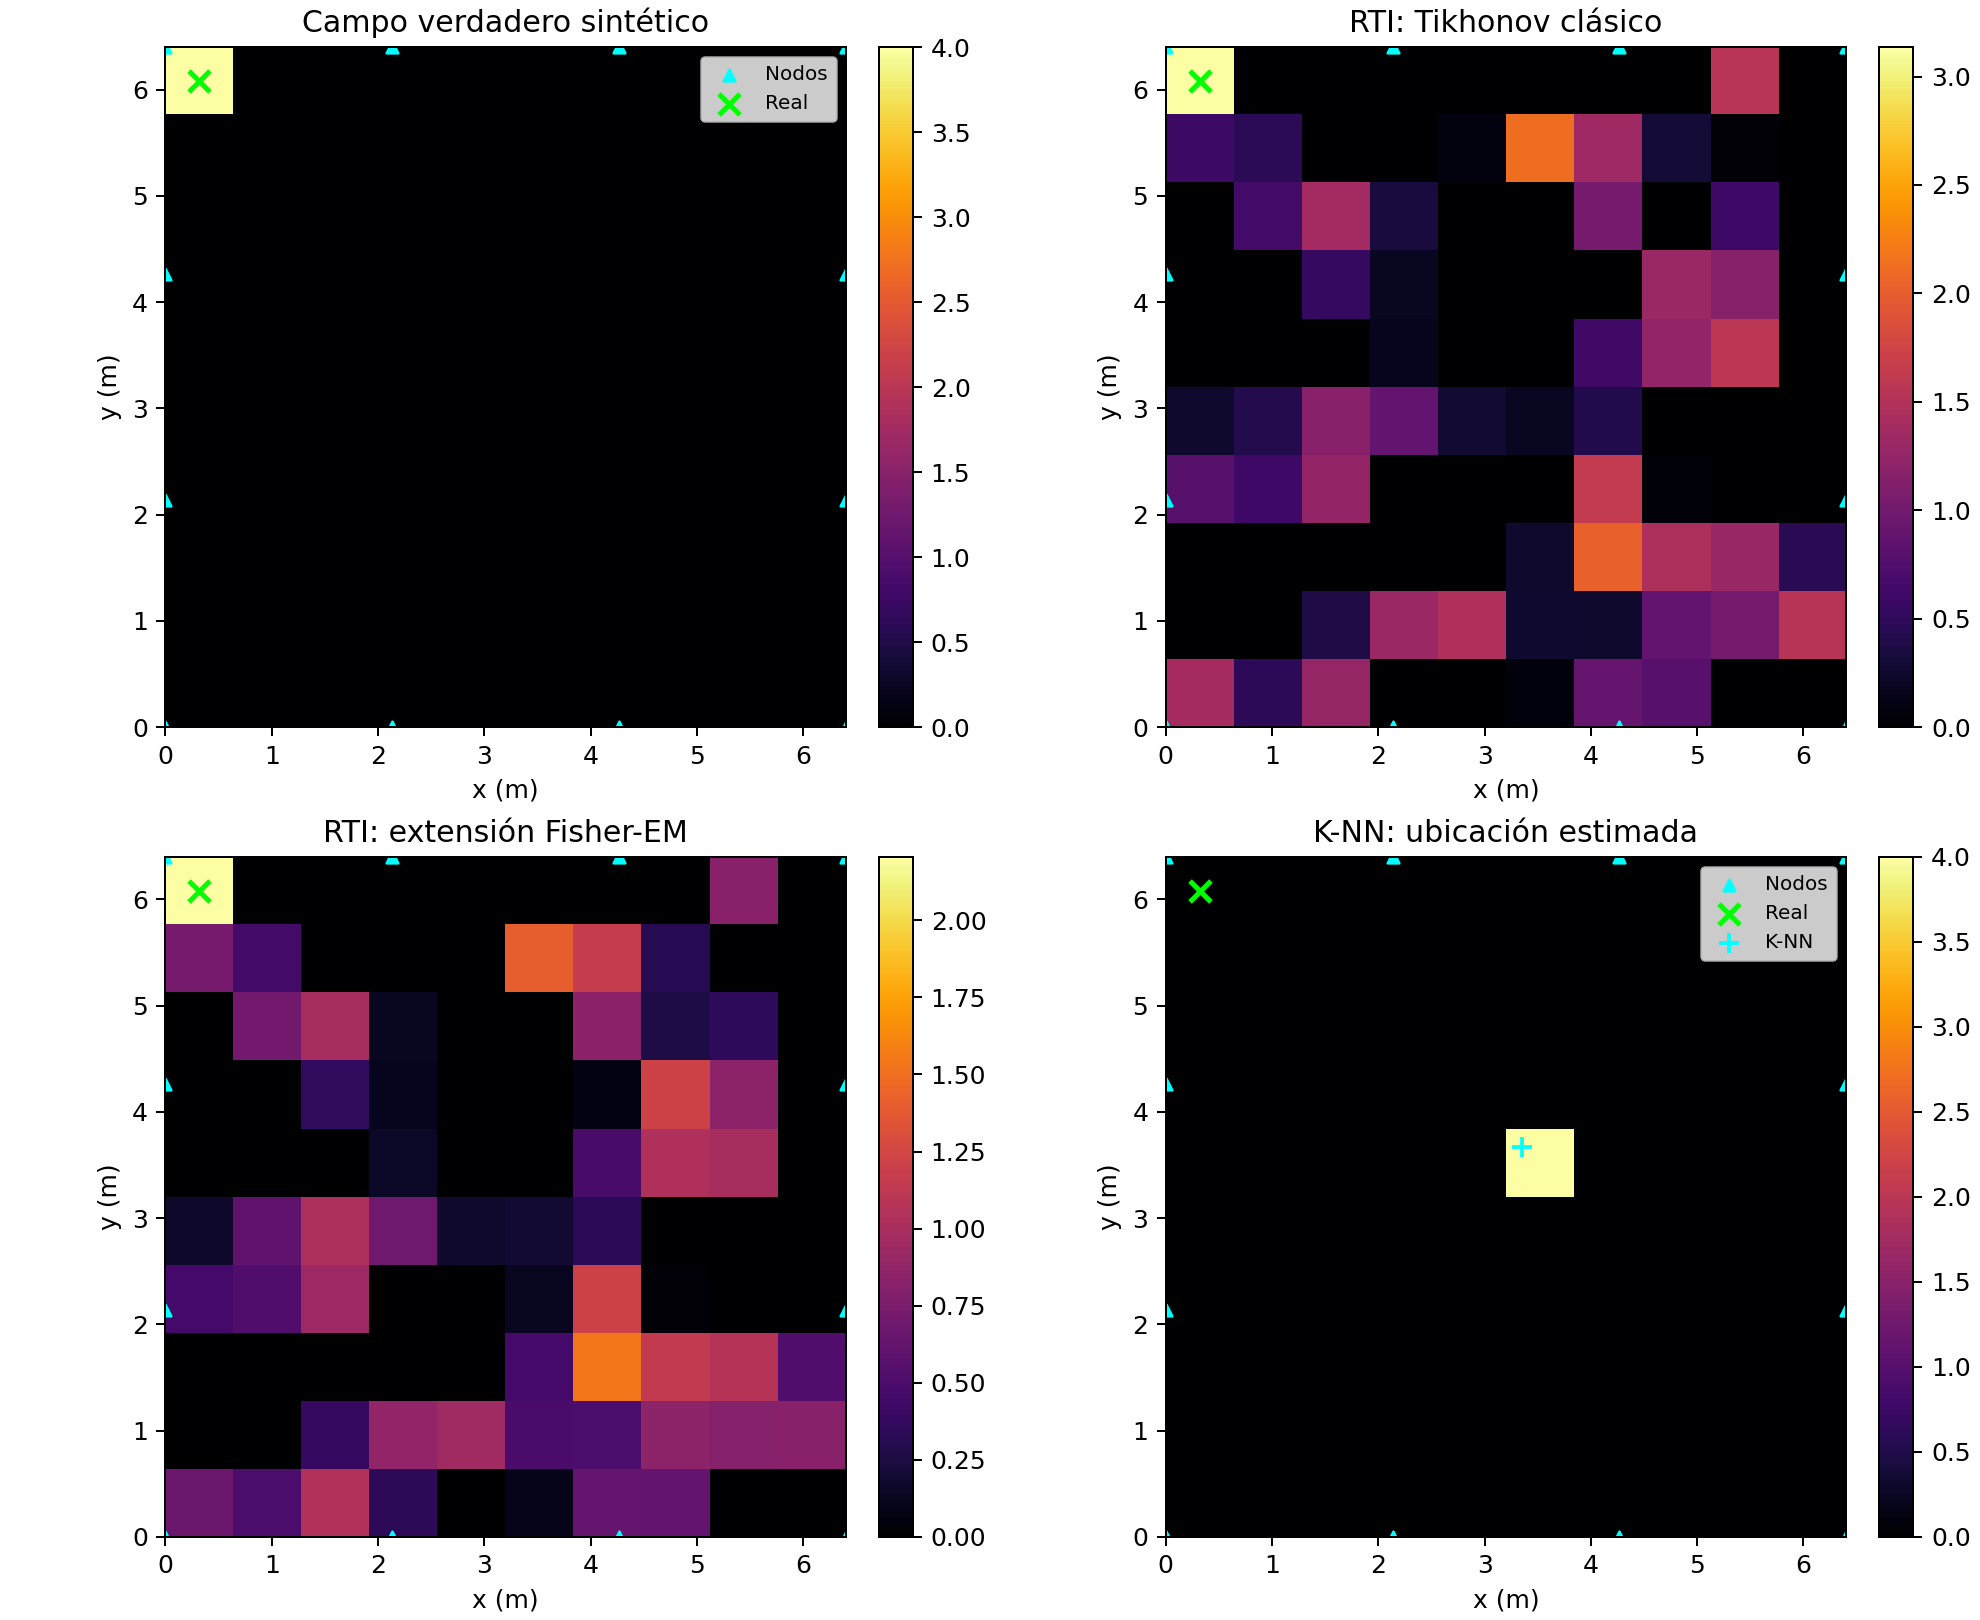
\includegraphics[width=.82\textwidth]{comparacion_rti_em_knn.png}
\caption{One illustrative generated case: true single-pixel image (top left), classical Tikhonov reconstruction (top right), scalar Fisher extension (bottom left), and weighted K-NN position (bottom right). The supplied source plot retains its Spanish labels. Color scales differ between panels, and the K-NN panel displays a coordinate prediction rather than a reconstructed attenuation field. This example is not an aggregate accuracy result. Source: the current preliminary-results comparison PNG.}
\label{fig:comparison}
\end{figure*}

\begin{figure}[t]
\centering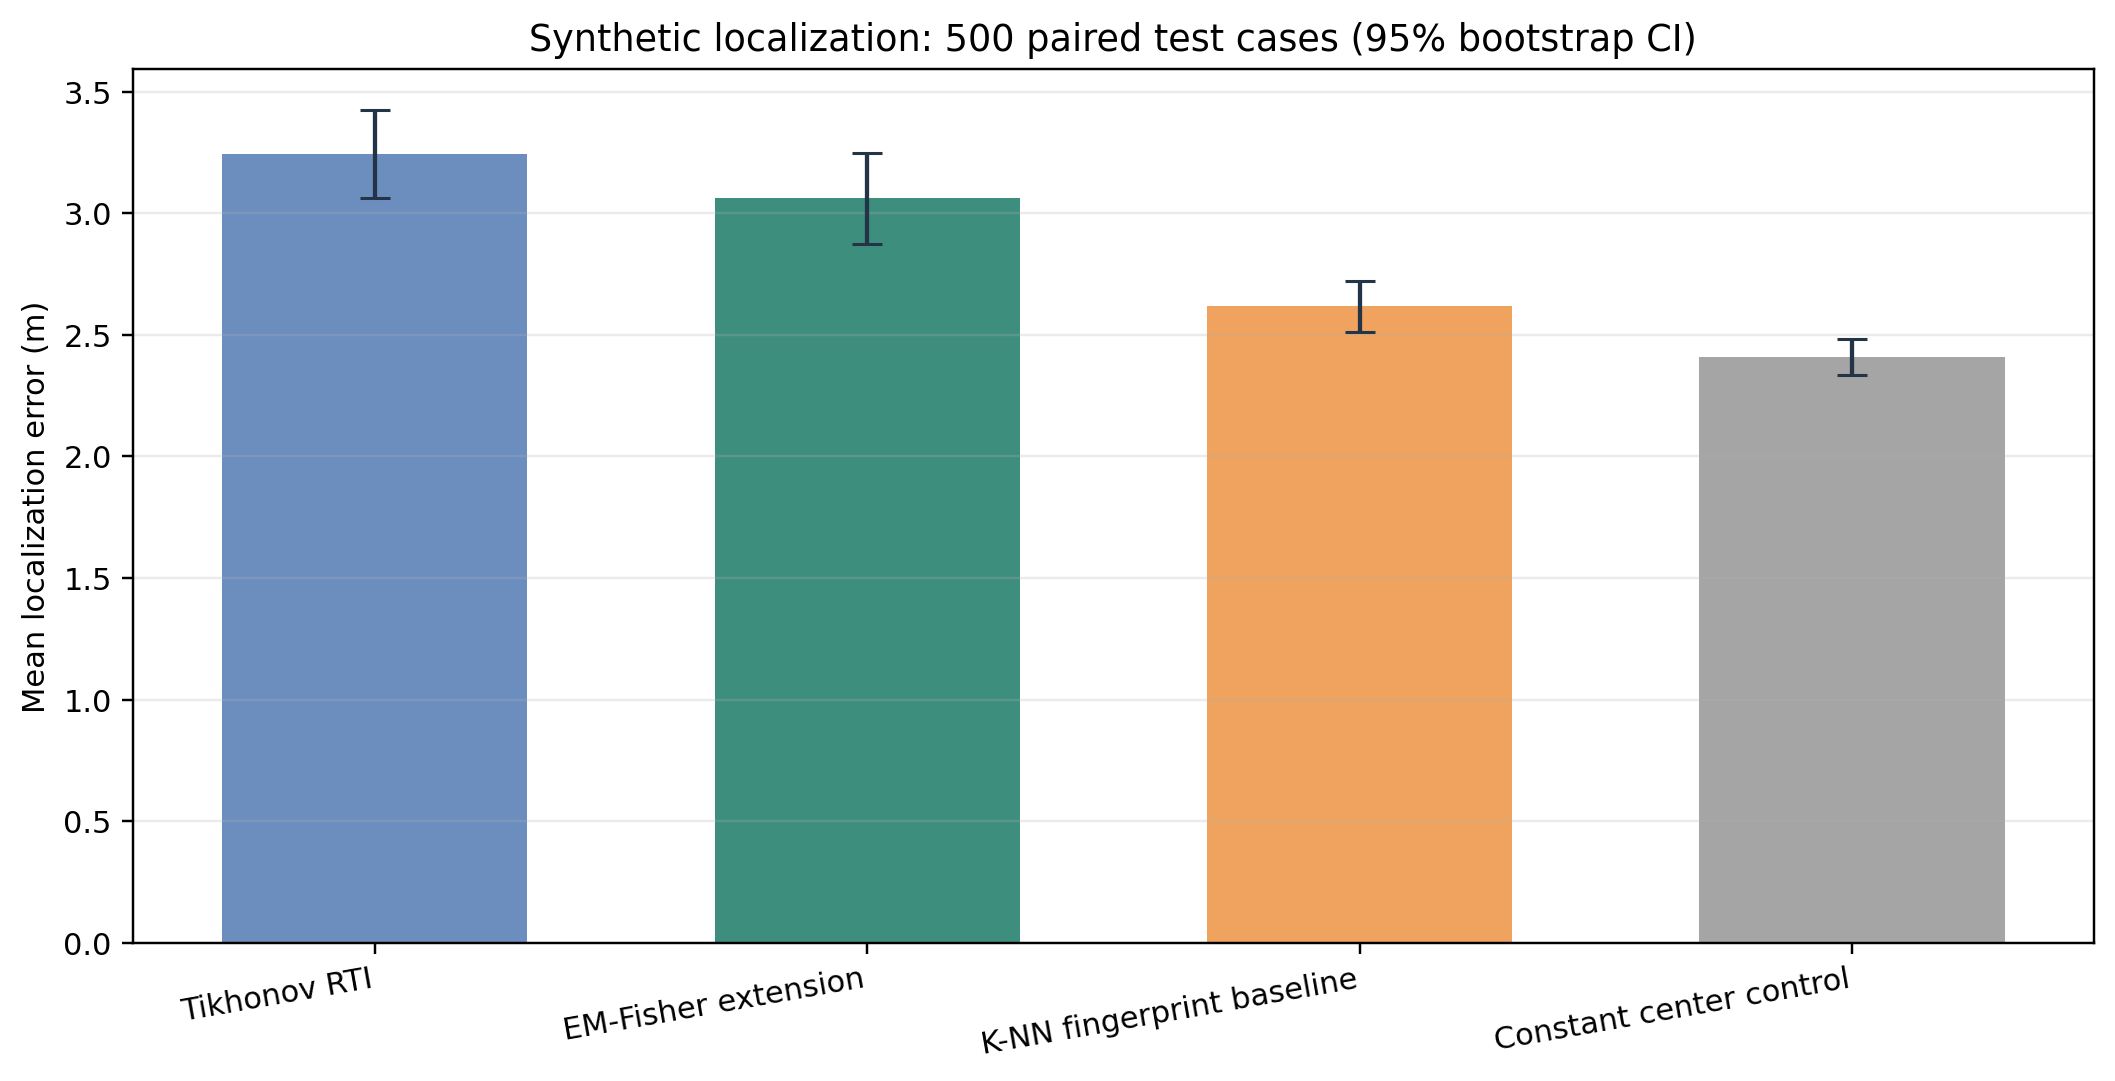
\includegraphics[width=\columnwidth]{localization_mean_error.png}
\caption{Mean position error on 500 paired synthetic cases; error bars are 95\% case-bootstrap intervals. The constant room-center control is included. Lower is better. Source: the current \texttt{metricas.csv} and its generated aggregate comparison plot.}
\label{fig:means}
\end{figure}

The classical RTI image MSE is .801107~dB$^2$, compared with .509575~dB$^2$ for the extension. These numbers concern map amplitudes averaged over pixels. Position error instead uses the maximum pixel. Smoothing can reduce an image-error metric while leaving a broad or incorrectly placed maximum. A map metric and a localization metric should therefore be reported together rather than substituted for one another.

The 95\% case-bootstrap interval for classical RTI mean error is [3.0642, 3.4228]~m; for the extension it is [2.8723, 3.2460]~m; and for weighted K-NN it is [2.5098, 2.7223]~m. These intervals quantify the stored generated cases under the conditioning described above. They should not be presented as uncertainty bounds for a deployed system.

\subsection{Paired comparisons}
The paired mean reduction from classical RTI to the extension is .182306~m, with a bootstrap interval [.067279, .299317]~m. The reduction from classical RTI to weighted K-NN is .625908~m, with interval [.420143, .832176]~m. From the extension to weighted K-NN it is .443602~m, with interval [.235722, .649831]~m. These positive intervals favor the stated candidates relative to their paired baselines on the generated cases.

They do not imply that the extension wins against a tuned Tikhonov family, that EM wins against K-NN, or that either method beats the no-signal control. The control is deliberately displayed in the main metric table and figure so that a favorable subset of pairwise comparisons cannot replace the full benchmark interpretation. The saved case-level predictions are the appropriate input for any additional paired comparison.

\section{Interpretation and Threats to Validity}
\subsection{What the EM result means}
The recovery experiment provides evidence that the implementation performs its intended restricted estimation task. It computes soft component assignments and updates a mixing probability and two second moments. Across the tested calibration sizes, its error generally decreases with more generated observations. That result is aligned with the assumptions of the experiment and can be defended without requiring EM to outperform an unrelated localization rule.

Parameter estimation and target localization have different ground truths. For calibration, the known parameters define an unambiguous recovery score. For localization, a fitted density is only one part of a pipeline that also depends on geometry, target representation, regularization, and the coordinate extraction rule. A well-fitted noise model cannot by itself correct a poor spatial forward model or a strongly biased position estimator.

\subsection{Why a scalar is insufficient for robustness}
The current $\gamma$ summarizes a density globally. It does not vary with the observed residual of a particular query link. Equation~\eqref{eq:equivalence} consequently places the extension inside the Tikhonov regularization family. The observed mean reduction is consistent with choosing a different smoothing strength. Attribution of this reduction specifically to latent mixture separation would require a comparison that controls for that strength.

A different future estimator could use the query residuals $y-Wx$ to compute posterior link responsibilities and update link-specific precisions while estimating the image. That would be another model and another iterative inverse problem. It is a proposed follow-up, not the estimator evaluated here. Its behavior under contamination would need to be measured, with clearly defined contamination and held-out configurations, before making a robustness claim.

Likewise, increasing the wide-component variance is only a statistical stress condition. It does not simulate a wall of a particular density, a moving reflector, a blocked link's packet loss, or coherent multipath. The appropriate language is ``generated mixture noise'' unless a physical propagation or measured-channel model supplies a more specific interpretation.

\subsection{Implication of the center-control result}
A bounded room offers prior positional information even without signals. Always predicting its center can have a moderate average error because every target is within a limited region. In this run, the signal-dependent methods do not convert observations into a lower mean distance error than that spatial prior. Their predictions may still differ case by case, but the principal reported utility metric does not favor them.

The deficit motivates inspecting case distributions and model settings before expanding to rescue scenarios. Potential contributors include the single-pixel target, sparse geometric sensitivity, noise amplitude relative to signal, smoothing choices, and the maximum-pixel rule. The current evidence does not isolate their relative contributions. Naming them as hypotheses is different from claiming to have diagnosed a measured radio failure.

Adding the control is an outcome of audit and strengthens the report's interpretability. It also prevents an assignment from requiring a predetermined ranking. If a course objective is to understand EM and evaluate an application, a negative application result can be informative when the algorithm, comparison, and limitations are correctly explained. The result should not be altered by selecting a seed or noise regime solely because it makes EM win.

\subsection{Comparison fairness and data leakage}
K-NN receives labeled references at every grid cell, including cells that can recur as test targets. Independent noise draws prevent identical training vectors, but the evaluation is spatially matched to the reference map. This is a legitimate matched-grid fingerprint test if described as such. It is not a held-out-position generalization test and should not be labeled one.

RTI uses a hand-selected ellipse width and smoothing coefficient, while K-NN uses a fixed neighborhood and three references per cell. None of these hyperparameters is selected through a separate development set in the current comparison. A fairer future study would allocate a development set, tune each method's parameters using only that set, and retain a test set untouched until the settings are fixed.

Equal test observations do not remove unequal setup requirements. A fingerprint database requires labeled positions; an RTI matrix requires surveyed geometry and a model. A future utility comparison should measure those acquisition and maintenance costs. The present synthetic generator makes both inexpensive to construct, so it cannot answer which approach would require less field work.

\subsection{Statistical and physical limitations}
The experiment uses one room geometry, one main calibration fit, one generating noise family, and one fixed main seed. Its 500 cases vary target selection and query noise within that configuration. Treating them as 500 independent building deployments would overstate the evidence. Replicating the entire calibration--training--query process across seeds would address a broader computational population, while real acquisition would address another level of external validity.

Noise is independent across links and draws. Actual RSS time series can be correlated, link-specific, quantized, censored by packet reception, and affected by transmitter power, antenna orientation, channel occupancy, and offsets. These effects can alter both the calibration distribution and the observation model. They are omitted rather than estimated implicitly.

The source's published $\gamma$ discrepancy also limits a claim of exact reproduction. This report reproduces the printed model formulas as interpreted in code and documents the numerical inconsistency. It does not resolve it by inventing precision, changing reported values, or equating the source's theoretical bound with the implemented image estimator.

\subsection{Timing limitations}
The local outputs contain exploratory timings. They are not used here to claim one method is faster. Dense RTI has precomputation, K-NN has reference construction, and EM calibration occurs before querying. The C++ EM diagnostic timers include process startup and serialization through the adapter; compilation is performed beforehand. Those times therefore do not isolate the cost of the C++ core. A meaningful comparison would define setup and inference consistently, warm the numerical libraries, repeat measurements, and report distributions under a controlled workload.

In particular, comparing precomputed RTI multiplication against an unprepared nearest-neighbor search measures a pipeline choice as well as an algorithm. The asymptotic analysis of the EM core remains valid as an operation-count statement. It should not be converted into a hardware-specific latency claim from a single run.

\section{A Focused Follow-up Protocol}
\subsection{Development and test separation}
The immediate computational follow-up should retain the current four methods and add the algebraically matched Tikhonov control. First define independent calibration, development, and test random streams. Use calibration only for noise fitting. Use development cases to choose $\alpha$, ellipse width, and K-NN settings. Freeze those choices before generating or opening test summaries.

Two spatial tasks should be distinguished. A matched-grid task allows test locations to have reference fingerprints, with independent noise draws. A held-out-position task excludes test positions from the fingerprint map and states how interpolation is assessed. Reporting them separately prevents a method's success under one task from being interpreted as performance under the other.

The first decision criterion is mean-distance improvement over the center control, accompanied by RMSE and a distribution of errors. The second is whether an EM-based method improves over an independently tuned Tikhonov method. The third is whether any improvement persists across full-pipeline repetitions, rather than a single favorable calibration fit. No numerical threshold is declared achieved by the present study.

\subsection{If calibration behavior is the main assignment}
For a short algorithms deliverable, EM recovery is already the clearest experiment. A follow-up can vary separation of the two spreads, narrow-component probability, sample size, initialization, or stopping tolerance while keeping the task identifiable. Each factor should have a stated hypothesis and its own table of recovered parameters and convergence behavior.

For example, bringing the two spreads close together reduces the practical distinction between components. It may become harder to recover the individual parameters even when the fitted density predicts held-out residuals reasonably well. Measuring both parameter error and predictive log likelihood would reveal that difference. This proposed experiment would teach a more precise limitation of mixture estimation than simply labeling a localization result as an EM success or failure.

Another useful comparison would fit a single zero-mean normal and the two-component mixture, then compare held-out residual likelihood. That comparison tests whether the added mixture flexibility improves prediction under specified conditions. It must use independent data because a more flexible model can improve training likelihood without improving future predictions. These are planned analyses, not reported results.

\subsection{If physical acquisition becomes available}
The first measurement session should use an open, bounded area with surveyed node positions and a stable set of links. Log timestamps, sender and receiver identifiers, RSS, channel, transmit power, packet success, and calibration state. Record an empty-area baseline before introducing a person at known positions. This establishes what the available hardware can actually measure before adding walls or obstacles.

Link-wise offset removal and exploratory distributions would then precede mixture fitting. Repeated sessions would allow a distinction between within-session noise and changes across sessions. Test positions and sessions should be held out according to the intended use. A physical experiment may show that another density, target model, or geometry is needed; preserving that possibility is part of evaluating the method.

Only after those checks would obstacle experiments be interpretable. An eventual search-and-rescue motivation requires substantially more evidence about propagation, availability of a baseline, deployment access, motion, false alarms, and field conditions. None of those requirements is resolved by the current synthetic parameter-recovery result.

\section{Reproducibility and Course Deliverables}
\subsection{Editable source and compilation}
This manuscript uses the official IEEEtran conference class and a continuous two-column LaTeX flow. The editable package contains \texttt{main.tex}, \texttt{refs.bib}, \texttt{enlaces.tex}, the figures, and the unmodified class and bibliography style. It can be uploaded to Overleaf with \texttt{main.tex} as the main document. The supplied Python compilation helper invokes a local LaTeX engine and packages those sources; it does not generate page images disguised as editable manuscript text.

The PDF is a course manuscript, not a published IEEE article or evidence of journal acceptance. The IEEE layout supports a clear technical presentation. The content and length follow the course deliverable, while source traceability and explicit limitations remain the author's responsibility.

\subsection{Reproduction sequence}
The assigned source is \texttt{em.cpp}, compiled as C++17. The auxiliary experiment command is \texttt{python simulacion\_rti\_em\_knn.py}, using the documented C++ backend defaults. The adapter executes the compiled EM routine for calibration and its repeated diagnostics. Python writes the local result tables, carries out the surrounding RTI computations, and produces comparison plots. A Python reference fit is available for implementation validation and is identified explicitly when selected.

The explicit build command is \texttt{python compilar\_cpp.py}; the helper invokes \texttt{g++} and records its actual flags and version. Running \texttt{build/em.exe --demo} executes the four-residual, one-iteration example in C++. The source requires only the C++ standard library. Its command-line fitting mode accepts residuals and initial settings, so the assigned algorithm can also be exercised independently of the RTI driver.

Rerunning the experiment overwrites generated outputs in the selected output directory, so an archived result snapshot should be kept when comparing manuscript versions. Reported numerical claims should always identify a single coherent run. The manuscript package preserves copies of its plotted figures, and its provenance note identifies their source files rather than synthesizing historical outcomes from different runs.

An independent reader can check the error table directly from saved predictions, the EM diagnostic table from its replicate summary, the mixture density from the fitted parameters, and the scalar equivalence by factoring $\gamma$ from the normal equations. These checks cover different failure modes and are more informative than treating the existence of a PDF as evidence that the computation is correct.

\subsection{Submission links and implementation language}
The course implementation of EM is C++17. The deliverable includes its editable source and a short explainable core for the oral defense. Auxiliary Python scripts support the synthetic application and numerical validation. This language division is stated explicitly so that execution of a Python experiment driver is not confused with the language implementing the assigned algorithm.

The author must complete and verify the manuscript, repository, and video URLs in the delivery appendix. Pending links are shown explicitly as text; no public repository, uploaded Overleaf project, or recorded presentation is invented. The editable source can be compiled before those external delivery steps are completed.

\section{Conclusion}
The restricted C++17 EM implementation recovers known mixture parameters with decreasing error as calibration sample size generally increases, and the tested random starts yield nearly identical estimates on one fixed sample. These are direct, reproducible findings about the algorithm under its own generating assumptions. The derivation and numerical example explain why responsibilities and weighted second moments produce those updates. Python utilities support the surrounding synthetic application and the reference cross-checks.

The localization result is substantially weaker. Mean errors are 3.244~m for classical Tikhonov RTI, 3.062~m for its scalar Fisher extension, 2.618~m for weighted K-NN, and 2.407~m for the constant room-center control. Every signal-dependent method loses to that control in mean error. Moreover, the scalar extension is exactly a Tikhonov regularization change after rescaling, so its improvement cannot be attributed to link-specific robustness or a new EM localization mechanism.

The defensible course contribution is a transparent study of EM noise calibration connected to a limited synthetic RTI application. Useful localization, real Wi-Fi sensing, NLoS robustness, missing-data reconstruction, and obstacle penetration remain unestablished. Independent parameter tuning and a control-aware follow-up should precede broader application claims.

\appendices
\section{The C++17 EM Core}
\label{app:code}
Listing~\ref{lst:em} contains the EM core extracted directly from \texttt{em.cpp}. It uses log-domain normalization, spread flooring, label ordering, and a relative-parameter stopping rule. The complete editable C++17 source is included as \texttt{codigo/em.cpp} in the manuscript package. It also contains the standard-library includes, result structure, command-line interface, and demonstration surrounding the core.

The four-sample worked example can be checked through the C++ demonstration using $(-3,-1,1,3)$ and exactly one iteration initialized at $(.5,1,3)$. A complete fit should use an adequate sample and the configured stopping rule. A four-observation illustration is not evidence of reliable calibration. The compiler and source hash are recorded alongside the generated results and in the report provenance manifest.

\begin{figure*}[t]
\lstinputlisting[language=C++,linewidth=\textwidth,caption={Executed C++17 EM core for two Gaussian components with means fixed at zero. Extracted from the packaged editable source.},label={lst:em}]{codigo/em_core.cpp}
\end{figure*}

\section{Equation-to-Code Explanation for the Defense}
The input vector contains observed residuals, and the three scalar state variables are the parameters being estimated. The code does not receive latent labels from the generator. In \texttt{responsibility}, \texttt{a} and \texttt{b} represent log component probabilities, \texttt{largest} stabilizes exponentiation, and \texttt{ea} and \texttt{eb} provide normalized exponential terms. The E-step stores the returned narrow-component probabilities in the \texttt{tau} vector.

In the M-step, \texttt{mass1} and \texttt{mass2} are fractional sample counts. An explicit loop accumulates \texttt{square\_sum1} and \texttt{square\_sum2}, the weighted squared residuals. Dividing by the masses gives component variances because the means are fixed at zero. The square roots restore the standard-deviation parameterization. The \texttt{change} calculation measures whether the three parameters have stabilized relative to their previous magnitudes.

The floor and probability clipping restrict the parameter domain. The component swap changes names rather than the density, provided the probability is complemented at the same time. The convergence flag indicates whether the requested stopping condition was satisfied; it does not replace examination of the fitted density, sample adequacy, or the likelihood surface.

A concise oral explanation can follow this sequence: identify observed residuals and hidden component labels; write the two density values for one residual; normalize them to obtain its responsibility; sum responsibilities and weighted squares; update the three parameters; repeat until stable. RTI geometry should be introduced afterward so the student can demonstrate the EM algorithm independently of the larger simulation driver.

\section{Artifact and Claim Traceability}
The following mapping identifies which file supports each main result. Paths are relative to the repository and refer to one current preliminary-results snapshot. It distinguishes a measured local computation from a source-paper statement and from an untested future proposal.

\begin{table}[h]
\caption{Traceability of numerical and methodological claims}
\centering\small
\begin{tabular}{@{}p{.38\columnwidth}p{.55\columnwidth}@{}}
\toprule
Claim or artifact & Evidence origin\\\midrule
Generating mixture values & Source table~1~\cite{wilson2010}; recorded parameter JSON\\
Main fitted parameters & \path{parametros.json}\\
Sample-size recovery & \path{em_sample_size.csv}\\
Initialization agreement & \path{em_initialization.csv}\\
Position mean and RMSE & \path{metricas.csv}; case predictions\\
Paired error reductions & \path{comparaciones_pareadas.csv}\\
Figure 4 example images & Preliminary-results comparison PNG\\
Figure 5 and center control & Aggregate error plot, metrics, predictions\\
$\alpha/\gamma$ equivalence & Algebra of Eqs.~\eqref{eq:fisheroperator}--\eqref{eq:equivalence}\\
Real obstacles or NLoS robustness & Not evaluated\\
Missing-RSS imputation & Not implemented\\
\bottomrule
\end{tabular}
\end{table}

The source of Fig.~\ref{fig:comparison} is the comparison PNG copied from the current preliminary-results directory at compilation. The recovery and initialization figures are copies of local plots backed by their named diagnostic CSV files. The bundle includes a provenance manifest containing source paths and hashes so a later figure change can be detected.

\section{Delivery Links}
\label{app:links}
The three fields below are the delivery endpoints to be completed by the author. The local manuscript and source bundle are available independently of whether these external URLs have been supplied. A pending field is not an asserted public upload.

\noindent\textbf{Overleaf manuscript:} \OverleafLink

\medskip\noindent\textbf{GitHub repository:} \GitHubLink

\medskip\noindent\textbf{Recorded presentation:} \VideoLink

\medskip
The completion keys are listed below. The file \texttt{enlaces.tex} stores these fields separately so verified URLs can be inserted and the manuscript rebuilt without changing the scientific text.
\begin{flushleft}\small\ttfamily
PENDIENTE\_ENLACE\_OVERLEAF\\
PENDIENTE\_ENLACE\_GITHUB\\
PENDIENTE\_ENLACE\_VIDEO
\end{flushleft}

\bibliographystyle{IEEEtran}
\bibliography{refs}
\end{document}
